% Options for packages loaded elsewhere
\PassOptionsToPackage{unicode}{hyperref}
\PassOptionsToPackage{hyphens}{url}
%
\documentclass[
]{book}
\usepackage{lmodern}
\usepackage{amssymb,amsmath}
\usepackage{ifxetex,ifluatex}
\ifnum 0\ifxetex 1\fi\ifluatex 1\fi=0 % if pdftex
  \usepackage[T1]{fontenc}
  \usepackage[utf8]{inputenc}
  \usepackage{textcomp} % provide euro and other symbols
\else % if luatex or xetex
  \usepackage{unicode-math}
  \defaultfontfeatures{Scale=MatchLowercase}
  \defaultfontfeatures[\rmfamily]{Ligatures=TeX,Scale=1}
\fi
% Use upquote if available, for straight quotes in verbatim environments
\IfFileExists{upquote.sty}{\usepackage{upquote}}{}
\IfFileExists{microtype.sty}{% use microtype if available
  \usepackage[]{microtype}
  \UseMicrotypeSet[protrusion]{basicmath} % disable protrusion for tt fonts
}{}
\makeatletter
\@ifundefined{KOMAClassName}{% if non-KOMA class
  \IfFileExists{parskip.sty}{%
    \usepackage{parskip}
  }{% else
    \setlength{\parindent}{0pt}
    \setlength{\parskip}{6pt plus 2pt minus 1pt}}
}{% if KOMA class
  \KOMAoptions{parskip=half}}
\makeatother
\usepackage{xcolor}
\IfFileExists{xurl.sty}{\usepackage{xurl}}{} % add URL line breaks if available
\IfFileExists{bookmark.sty}{\usepackage{bookmark}}{\usepackage{hyperref}}
\hypersetup{
  pdftitle={A Minimal Book Example},
  pdfauthor={Yihui Xie},
  hidelinks,
  pdfcreator={LaTeX via pandoc}}
\urlstyle{same} % disable monospaced font for URLs
\usepackage{color}
\usepackage{fancyvrb}
\newcommand{\VerbBar}{|}
\newcommand{\VERB}{\Verb[commandchars=\\\{\}]}
\DefineVerbatimEnvironment{Highlighting}{Verbatim}{commandchars=\\\{\}}
% Add ',fontsize=\small' for more characters per line
\usepackage{framed}
\definecolor{shadecolor}{RGB}{248,248,248}
\newenvironment{Shaded}{\begin{snugshade}}{\end{snugshade}}
\newcommand{\AlertTok}[1]{\textcolor[rgb]{0.94,0.16,0.16}{#1}}
\newcommand{\AnnotationTok}[1]{\textcolor[rgb]{0.56,0.35,0.01}{\textbf{\textit{#1}}}}
\newcommand{\AttributeTok}[1]{\textcolor[rgb]{0.77,0.63,0.00}{#1}}
\newcommand{\BaseNTok}[1]{\textcolor[rgb]{0.00,0.00,0.81}{#1}}
\newcommand{\BuiltInTok}[1]{#1}
\newcommand{\CharTok}[1]{\textcolor[rgb]{0.31,0.60,0.02}{#1}}
\newcommand{\CommentTok}[1]{\textcolor[rgb]{0.56,0.35,0.01}{\textit{#1}}}
\newcommand{\CommentVarTok}[1]{\textcolor[rgb]{0.56,0.35,0.01}{\textbf{\textit{#1}}}}
\newcommand{\ConstantTok}[1]{\textcolor[rgb]{0.00,0.00,0.00}{#1}}
\newcommand{\ControlFlowTok}[1]{\textcolor[rgb]{0.13,0.29,0.53}{\textbf{#1}}}
\newcommand{\DataTypeTok}[1]{\textcolor[rgb]{0.13,0.29,0.53}{#1}}
\newcommand{\DecValTok}[1]{\textcolor[rgb]{0.00,0.00,0.81}{#1}}
\newcommand{\DocumentationTok}[1]{\textcolor[rgb]{0.56,0.35,0.01}{\textbf{\textit{#1}}}}
\newcommand{\ErrorTok}[1]{\textcolor[rgb]{0.64,0.00,0.00}{\textbf{#1}}}
\newcommand{\ExtensionTok}[1]{#1}
\newcommand{\FloatTok}[1]{\textcolor[rgb]{0.00,0.00,0.81}{#1}}
\newcommand{\FunctionTok}[1]{\textcolor[rgb]{0.00,0.00,0.00}{#1}}
\newcommand{\ImportTok}[1]{#1}
\newcommand{\InformationTok}[1]{\textcolor[rgb]{0.56,0.35,0.01}{\textbf{\textit{#1}}}}
\newcommand{\KeywordTok}[1]{\textcolor[rgb]{0.13,0.29,0.53}{\textbf{#1}}}
\newcommand{\NormalTok}[1]{#1}
\newcommand{\OperatorTok}[1]{\textcolor[rgb]{0.81,0.36,0.00}{\textbf{#1}}}
\newcommand{\OtherTok}[1]{\textcolor[rgb]{0.56,0.35,0.01}{#1}}
\newcommand{\PreprocessorTok}[1]{\textcolor[rgb]{0.56,0.35,0.01}{\textit{#1}}}
\newcommand{\RegionMarkerTok}[1]{#1}
\newcommand{\SpecialCharTok}[1]{\textcolor[rgb]{0.00,0.00,0.00}{#1}}
\newcommand{\SpecialStringTok}[1]{\textcolor[rgb]{0.31,0.60,0.02}{#1}}
\newcommand{\StringTok}[1]{\textcolor[rgb]{0.31,0.60,0.02}{#1}}
\newcommand{\VariableTok}[1]{\textcolor[rgb]{0.00,0.00,0.00}{#1}}
\newcommand{\VerbatimStringTok}[1]{\textcolor[rgb]{0.31,0.60,0.02}{#1}}
\newcommand{\WarningTok}[1]{\textcolor[rgb]{0.56,0.35,0.01}{\textbf{\textit{#1}}}}
\usepackage{longtable,booktabs}
% Correct order of tables after \paragraph or \subparagraph
\usepackage{etoolbox}
\makeatletter
\patchcmd\longtable{\par}{\if@noskipsec\mbox{}\fi\par}{}{}
\makeatother
% Allow footnotes in longtable head/foot
\IfFileExists{footnotehyper.sty}{\usepackage{footnotehyper}}{\usepackage{footnote}}
\makesavenoteenv{longtable}
\usepackage{graphicx,grffile}
\makeatletter
\def\maxwidth{\ifdim\Gin@nat@width>\linewidth\linewidth\else\Gin@nat@width\fi}
\def\maxheight{\ifdim\Gin@nat@height>\textheight\textheight\else\Gin@nat@height\fi}
\makeatother
% Scale images if necessary, so that they will not overflow the page
% margins by default, and it is still possible to overwrite the defaults
% using explicit options in \includegraphics[width, height, ...]{}
\setkeys{Gin}{width=\maxwidth,height=\maxheight,keepaspectratio}
% Set default figure placement to htbp
\makeatletter
\def\fps@figure{htbp}
\makeatother
\setlength{\emergencystretch}{3em} % prevent overfull lines
\providecommand{\tightlist}{%
  \setlength{\itemsep}{0pt}\setlength{\parskip}{0pt}}
\setcounter{secnumdepth}{5}
\usepackage{booktabs}
\usepackage{amsthm}
\makeatletter
\def\thm@space@setup{%
  \thm@preskip=8pt plus 2pt minus 4pt
  \thm@postskip=\thm@preskip
}
\makeatother
\usepackage[]{natbib}
\bibliographystyle{plainnat}

\title{A Minimal Book Example}
\author{Yihui Xie}
\date{2020-12-03}

\begin{document}
\maketitle

{
\setcounter{tocdepth}{1}
\tableofcontents
}
\hypertarget{prerequisites}{%
\chapter{Prerequisites}\label{prerequisites}}

This is a \emph{sample} book written in \textbf{Markdown}. You can use anything that Pandoc's Markdown supports, e.g., a math equation \(a^2 + b^2 = c^2\).

The \textbf{bookdown} package can be installed from CRAN or Github:

\begin{Shaded}
\begin{Highlighting}[]
\KeywordTok{install.packages}\NormalTok{(}\StringTok{"bookdown"}\NormalTok{)}
\CommentTok{# or the development version}
\CommentTok{# devtools::install_github("rstudio/bookdown")}
\end{Highlighting}
\end{Shaded}

Remember each Rmd file contains one and only one chapter, and a chapter is defined by the first-level heading \texttt{\#}.

To compile this example to PDF, you need XeLaTeX. You are recommended to install TinyTeX (which includes XeLaTeX): \url{https://yihui.name/tinytex/}.

\hypertarget{the-whole-document-lol}{%
\chapter{The whole document lol}\label{the-whole-document-lol}}

\hypertarget{quick-overview-of-race-and-rurality}{%
\chapter{Quick overview of Race and Rurality}\label{quick-overview-of-race-and-rurality}}

\hypertarget{sample-sizesdistributions}{%
\section{Sample sizes/Distributions}\label{sample-sizesdistributions}}

Let's kick it off with a quick overview of distribution of race and rurality and their intersection.

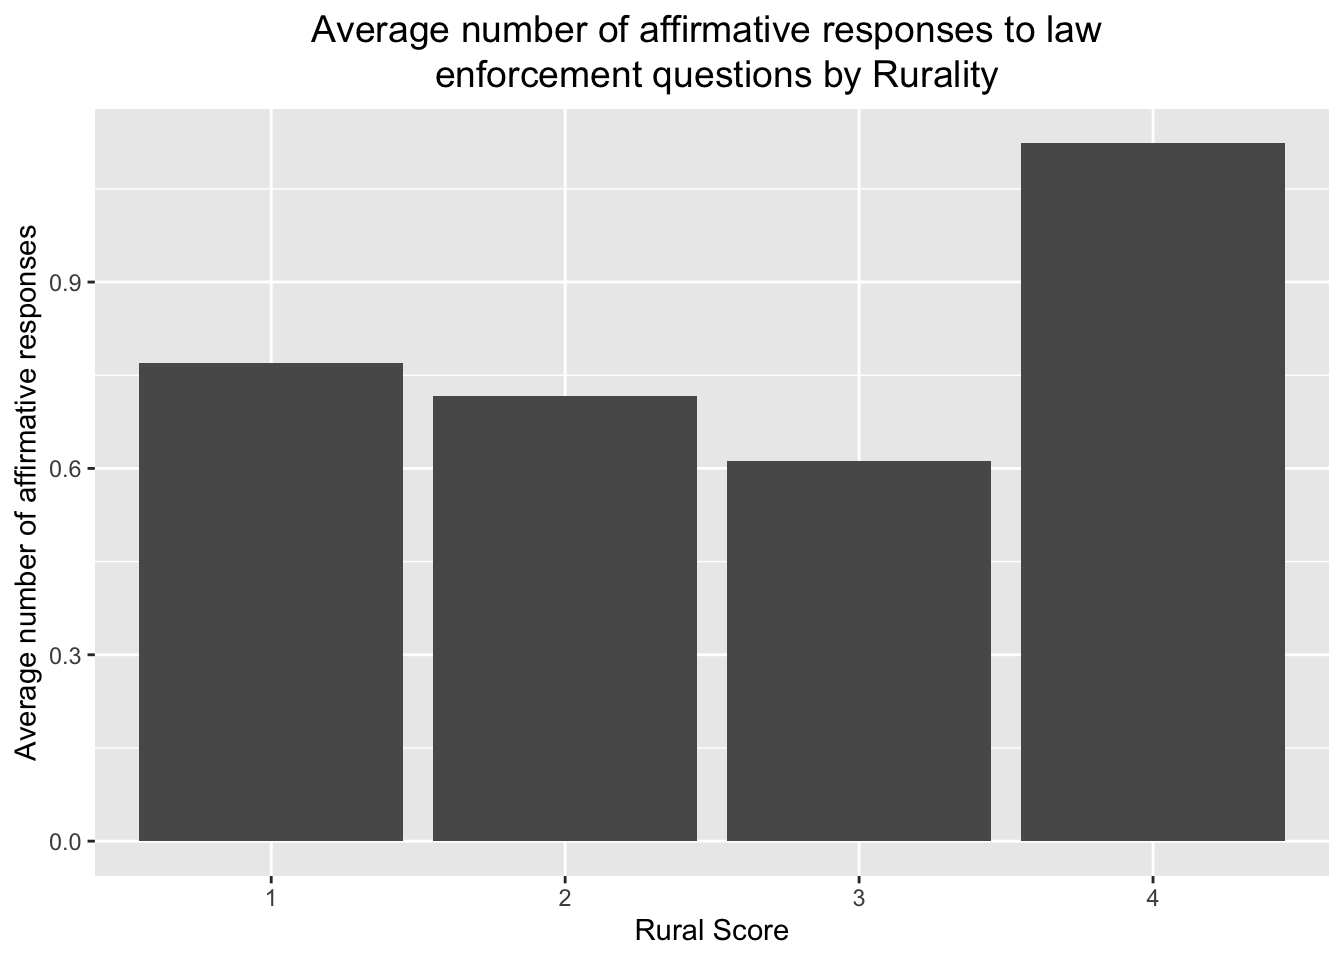
\includegraphics{coocli_files/figure-latex/unnamed-chunk-4-1.pdf}

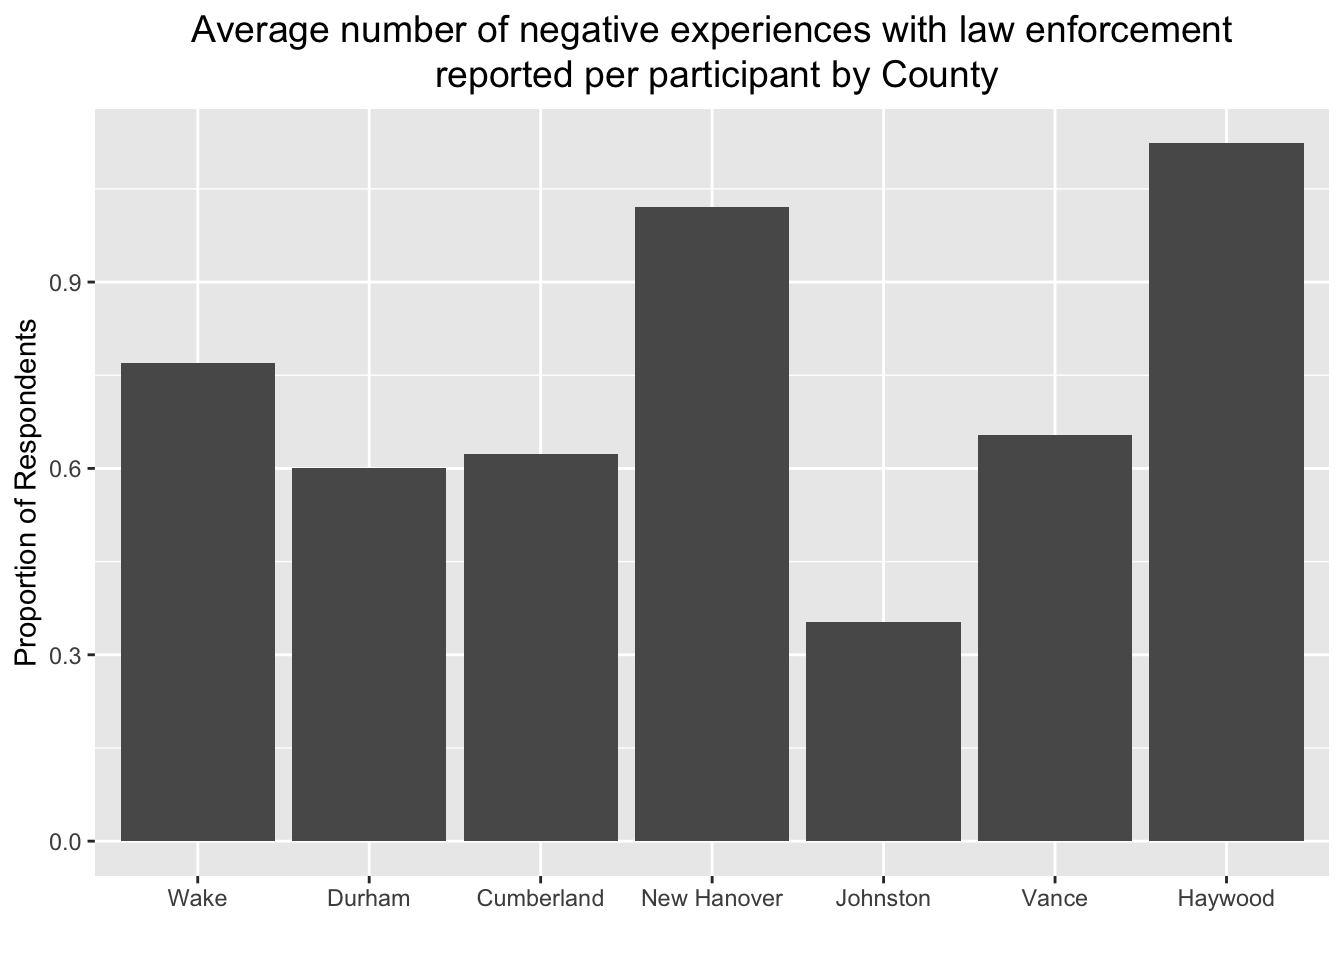
\includegraphics{coocli_files/figure-latex/unnamed-chunk-5-1.pdf}

\hypertarget{of-the-durham-participants-surveyed-were-black.-this-may-have-skewed-the-racial-distribution-in-durham-but-provided-a-significant-boost-to-the-representation-of-black-americans-in-the-survey-overall-given-that-59-66-of-the-89-african-americans-who-responded-to-our-survey-were-from-durham.}{%
\subsection{74\% of the Durham participants surveyed were black. This may have skewed the racial distribution in Durham, but provided a significant boost to the representation of black Americans in the survey overall, given that 59 (66\%) of the 89 African Americans who responded to our survey were from Durham.}\label{of-the-durham-participants-surveyed-were-black.-this-may-have-skewed-the-racial-distribution-in-durham-but-provided-a-significant-boost-to-the-representation-of-black-americans-in-the-survey-overall-given-that-59-66-of-the-89-african-americans-who-responded-to-our-survey-were-from-durham.}}

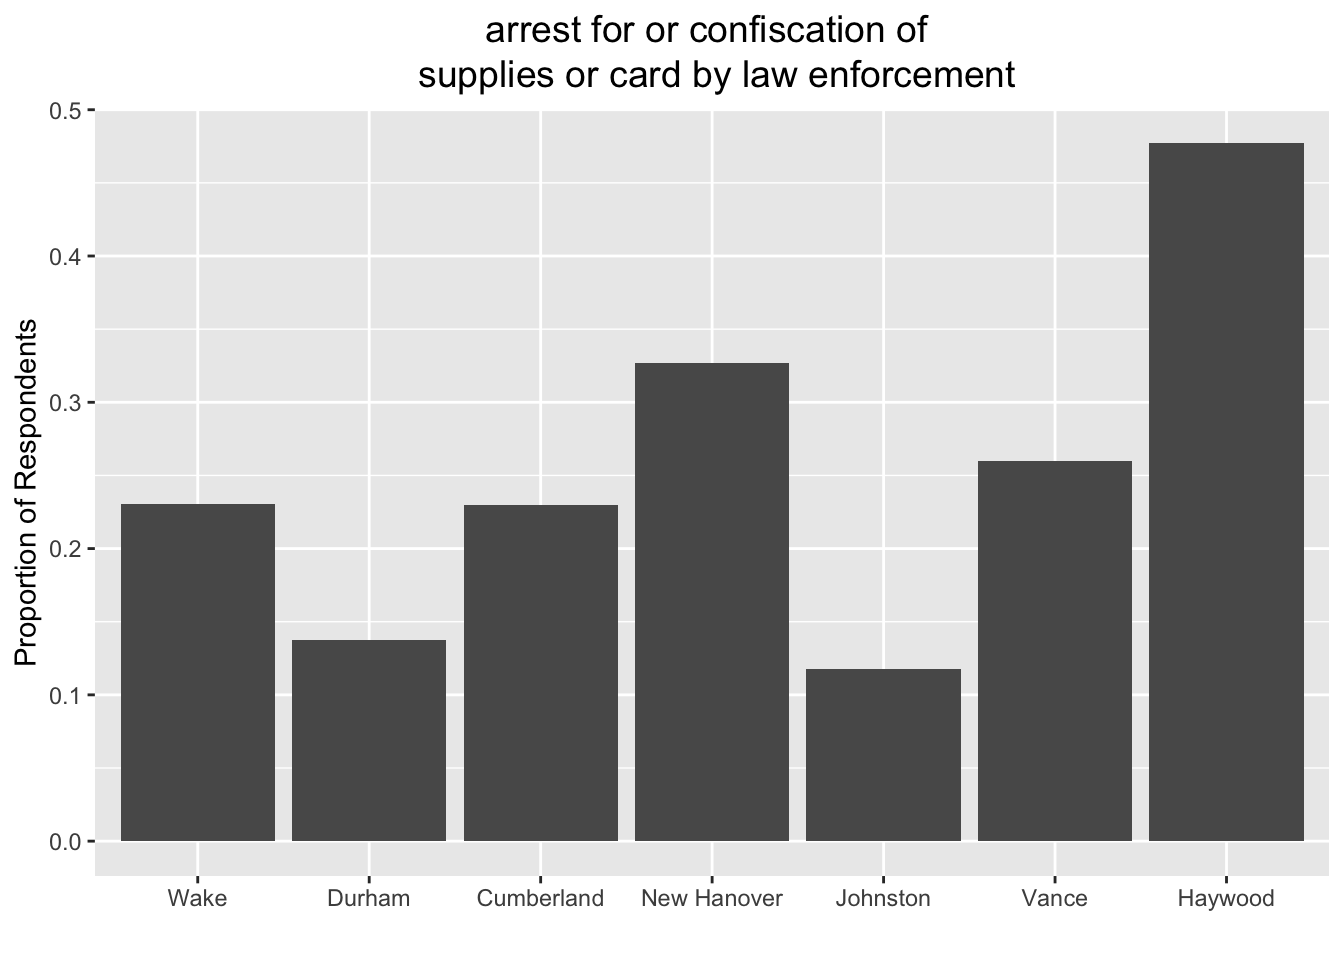
\includegraphics{coocli_files/figure-latex/unnamed-chunk-6-1.pdf} 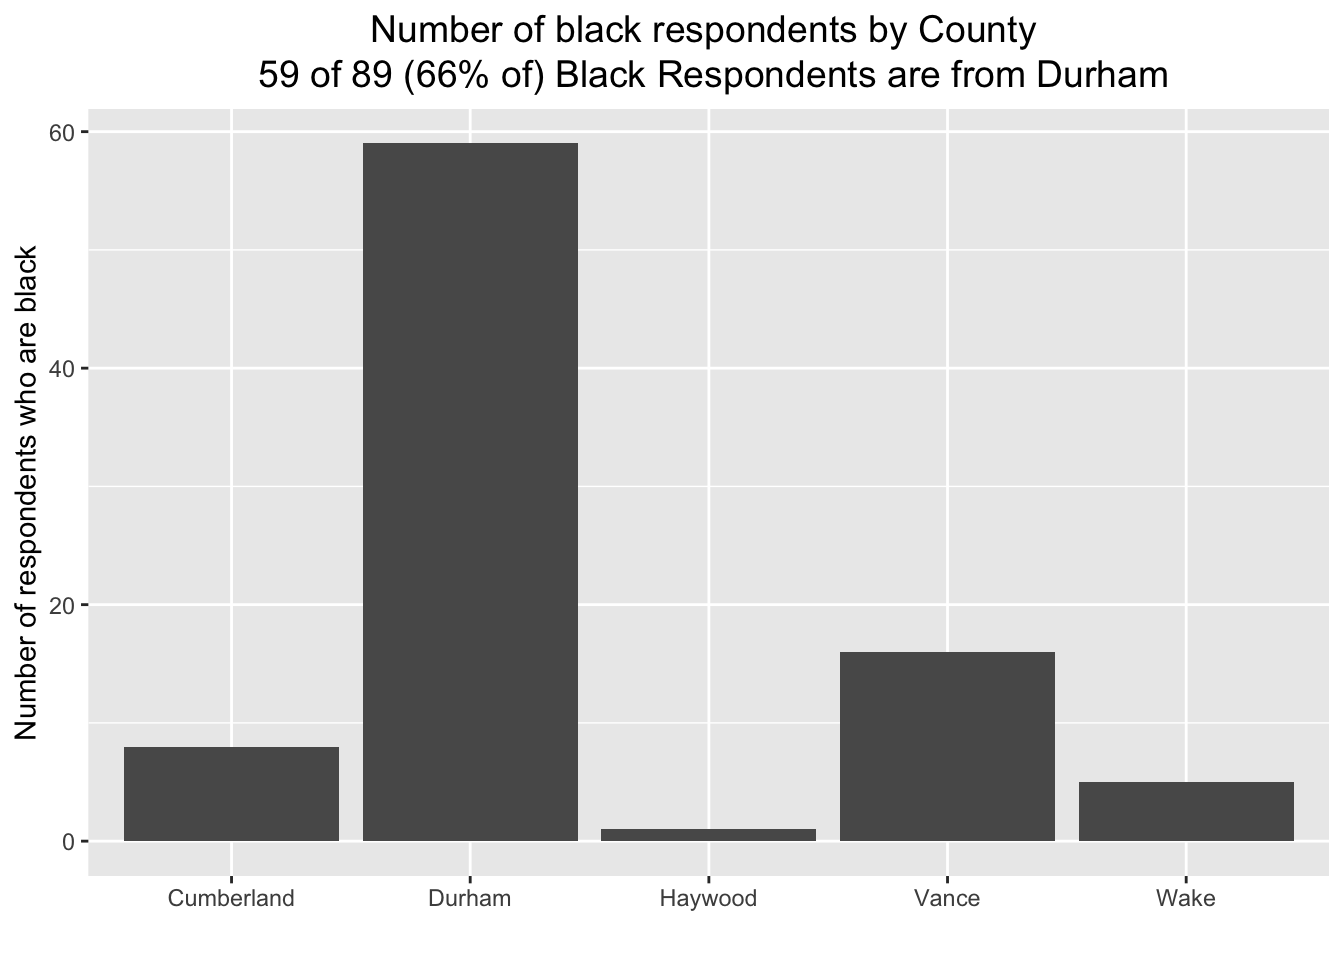
\includegraphics{coocli_files/figure-latex/unnamed-chunk-6-2.pdf}

\hypertarget{rurality-and-statements-about-law-enforcement}{%
\chapter{Rurality and Statements about Law Enforcement}\label{rurality-and-statements-about-law-enforcement}}

The variable across the columns here is the \emph{sum} of the responses to the questions about law enforcement. To test the significance of this, we can use Kruskal-Wallis on the lawSum variable or consider a chi-square test on the binary attribute I(lawSum\textgreater0).

\hypertarget{significant-differences-in-the-overall-number-of-statements-about-law-enforcement-identified-across-levels-of-rurality.}{%
\subsection{Significant differences in the overall number of statements about law Enforcement identified across levels of rurality.}\label{significant-differences-in-the-overall-number-of-statements-about-law-enforcement-identified-across-levels-of-rurality.}}

\hypertarget{the-number-of-participants-identifying-with-at-least-one-statement-regarding-law-enforcement-does-appear-to-have-an-ordinal-relationship-with-rurality.}{%
\subsubsection{\texorpdfstring{The number of participants identifying with \emph{at least one} statement regarding Law Enforcement does appear to have an ordinal relationship with rurality.}{The number of participants identifying with at least one statement regarding Law Enforcement does appear to have an ordinal relationship with rurality.}}\label{the-number-of-participants-identifying-with-at-least-one-statement-regarding-law-enforcement-does-appear-to-have-an-ordinal-relationship-with-rurality.}}

And for many reasons this is a good measurement of \emph{breadth} of a problem with law enforcement (a number not influenced by a ``few excessive complainers'').

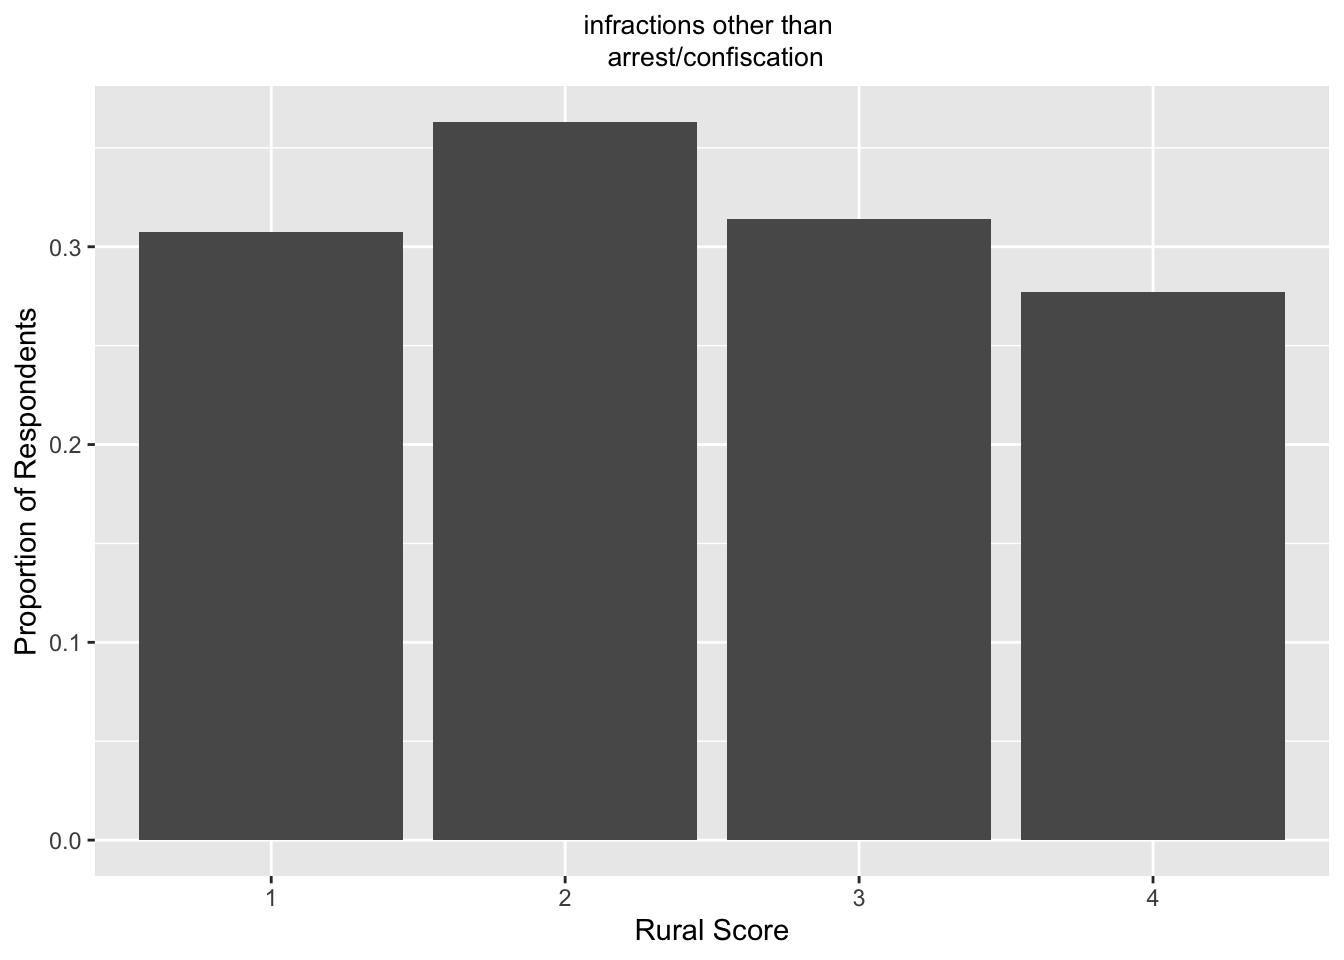
\includegraphics{coocli_files/figure-latex/unnamed-chunk-7-1.pdf}

\begin{verbatim}
##            Chisq Df       Prob
## cor     3.698450  1 0.05446305
## rmeans  5.999568  3 0.11163122
## cmeans  3.698450  1 0.05446305
## general 5.999568  3 0.11163122
\end{verbatim}

The first row of this table gives us rationale to gather more data - as there does appear to be some linear relationship here but as we will see in the next section, that relationship disappears after the removal of a few key questions in Haywood county.

\hypertarget{diving-deeper-we-see-that-the-average-number-of-complaints-involving-law-enforcement-do-not-follow-the-same-pattern.-although-youll-notice-that-in-haywood-thatd-be-rural-score-4-complaints-averaged-over-1-per-survey-response-which-is-notable-given-the-distribution-of-responses-across-the-other-rural-scores.-when-we-compare-haywood-on-a-county-level-we-find-only-new-hanover-can-begin-to-compete-with-most-other-counties-averaging-fewer-than-0.7-complaints-per-response.}{%
\subsubsection{\texorpdfstring{Diving Deeper, we see that the average \emph{number of complaints} involving law enforcement do not follow the same pattern. Although you'll notice that in Haywood (that'd be rural score = 4) complaints averaged over 1 per survey response, which is notable given the distribution of responses across the other rural scores. When we compare Haywood on a county level, we find only New Hanover can begin to compete, with most other counties averaging fewer than 0.7 complaints per response.}{Diving Deeper, we see that the average number of complaints involving law enforcement do not follow the same pattern. Although you'll notice that in Haywood (that'd be rural score = 4) complaints averaged over 1 per survey response, which is notable given the distribution of responses across the other rural scores. When we compare Haywood on a county level, we find only New Hanover can begin to compete, with most other counties averaging fewer than 0.7 complaints per response.}}\label{diving-deeper-we-see-that-the-average-number-of-complaints-involving-law-enforcement-do-not-follow-the-same-pattern.-although-youll-notice-that-in-haywood-thatd-be-rural-score-4-complaints-averaged-over-1-per-survey-response-which-is-notable-given-the-distribution-of-responses-across-the-other-rural-scores.-when-we-compare-haywood-on-a-county-level-we-find-only-new-hanover-can-begin-to-compete-with-most-other-counties-averaging-fewer-than-0.7-complaints-per-response.}}

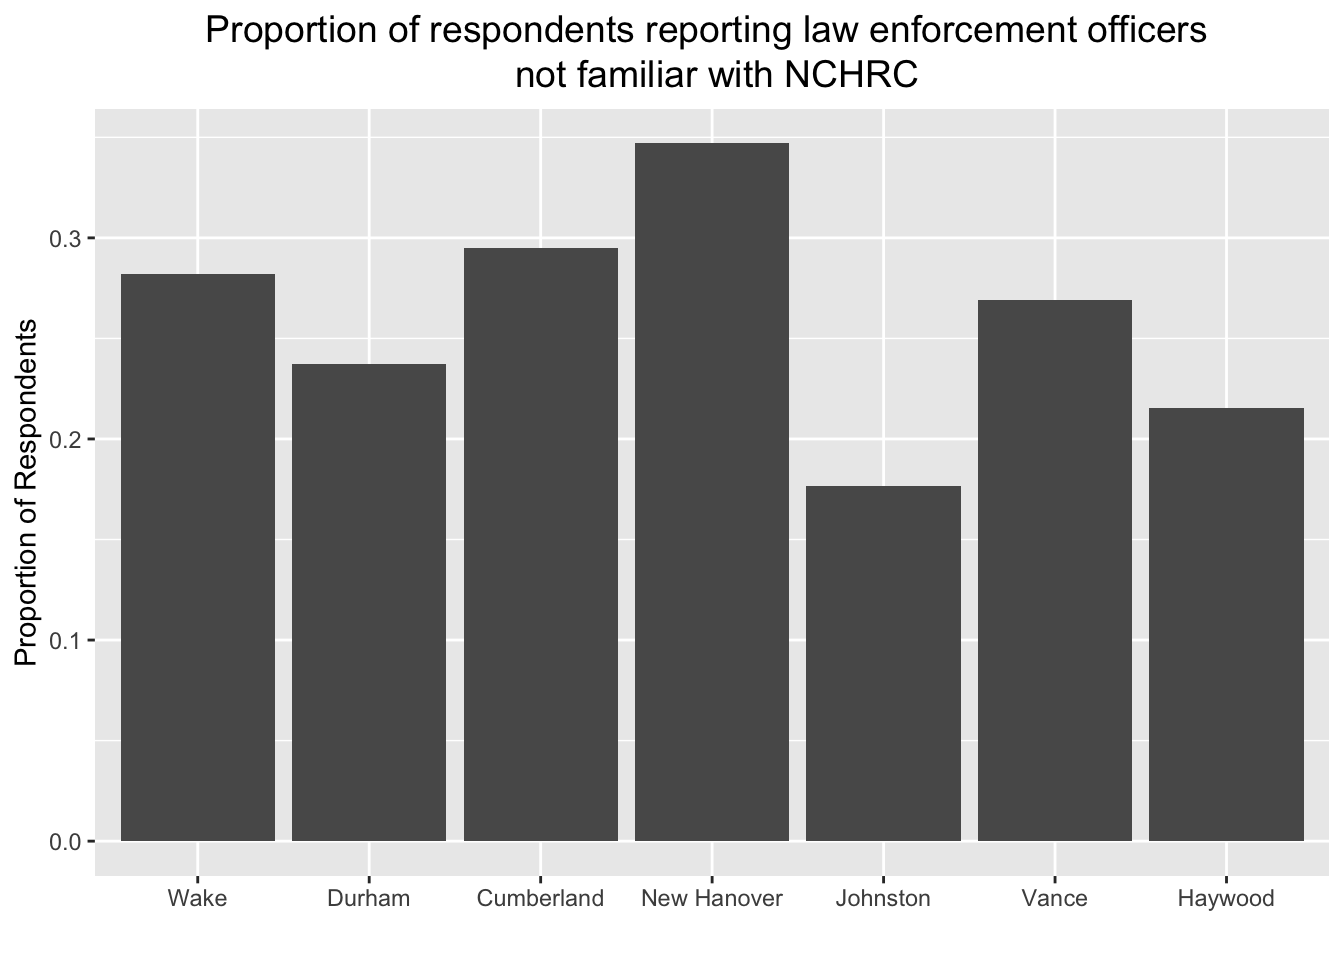
\includegraphics{coocli_files/figure-latex/unnamed-chunk-8-1.pdf}

\begin{verbatim}
## 
##  Kruskal-Wallis rank sum test
## 
## data:  lawSum by rural.fac
## Kruskal-Wallis chi-squared = 8.5482, df = 3, p-value = 0.03594
\end{verbatim}

\begin{verbatim}
##             Chisq Df       Prob
## cor      3.060855  1 0.08019947
## rmeans  11.703664  3 0.00847039
## cmeans   5.776325  5 0.32859550
## general 22.855603 15 0.08725417
\end{verbatim}

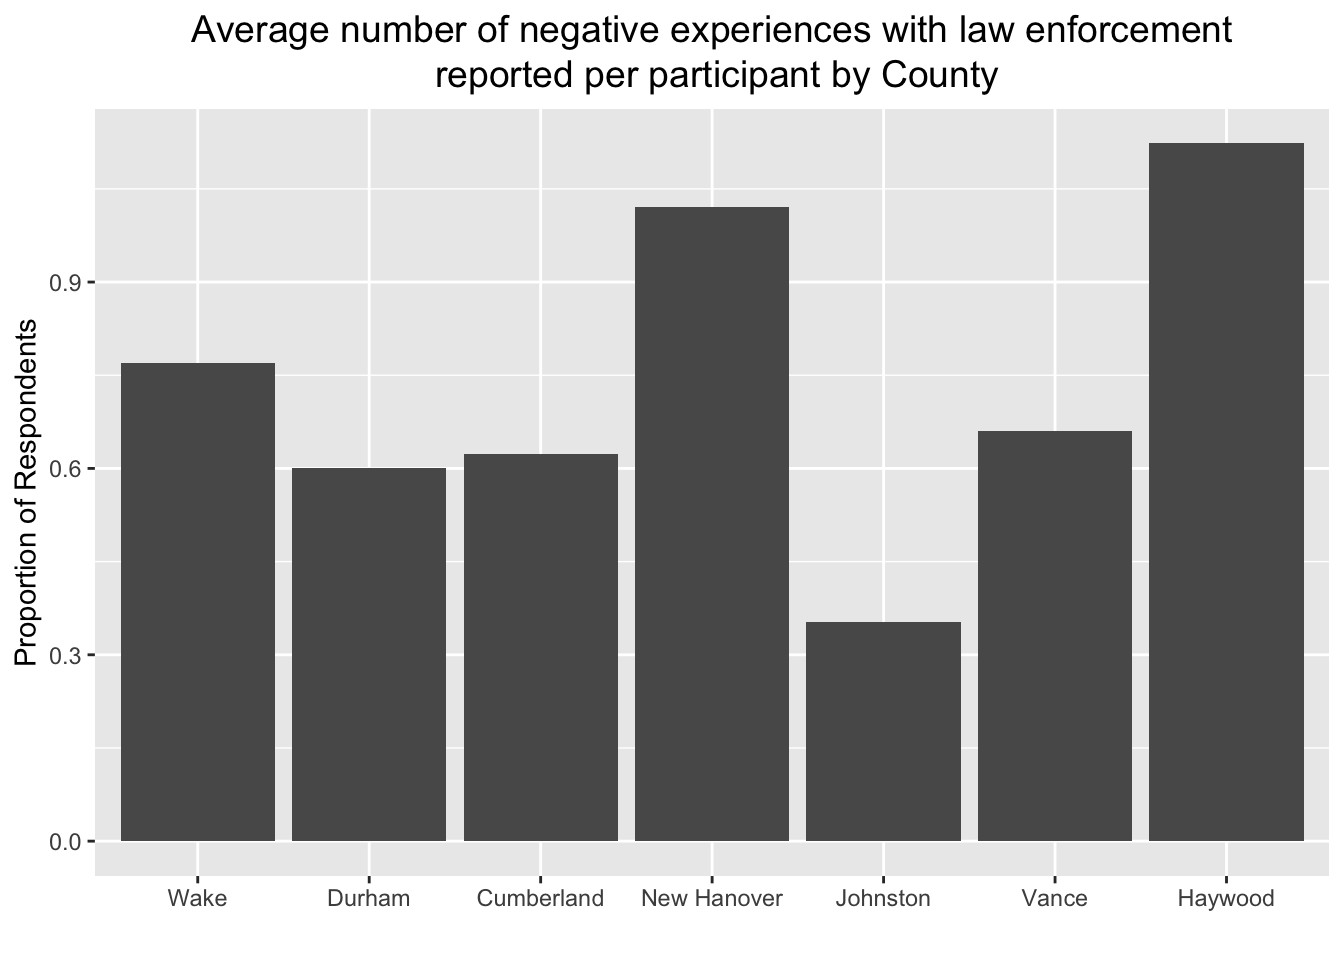
\includegraphics{coocli_files/figure-latex/unnamed-chunk-8-2.pdf}

\hypertarget{the-connection-between-rurality-and-infractions-by-law-enforcement-officers-is-driven-by-the-outrageous-frequency-of-arrests-and-confiscations-in-haywood.-nearly-half-of-the-65-respondents-from-haywood-reported-either-confiscation-of-or-arrest-for-supplies-they-received-legally-from-nchrc.-this-is-in-fact-the-one-thing-separating-haywood-from-the-other-counties.-once-these-questions-are-removed-from-the-analysis-no-significant-relationship-with-rurality-remains.}{%
\section{\texorpdfstring{The connection between rurality and infractions by law enforcement officers is driven by the \emph{outrageous} frequency of arrests and confiscations in Haywood. Nearly \emph{half} of the 65 respondents from Haywood reported \emph{either \emph{confiscation of} or \emph{arrest for}} supplies they received legally from NCHRC. This is in fact the one thing separating Haywood from the other counties. Once these questions are removed from the analysis, no significant relationship with rurality remains.}{The connection between rurality and infractions by law enforcement officers is driven by the outrageous frequency of arrests and confiscations in Haywood. Nearly half of the 65 respondents from Haywood reported either confiscation of or arrest for supplies they received legally from NCHRC. This is in fact the one thing separating Haywood from the other counties. Once these questions are removed from the analysis, no significant relationship with rurality remains.}}\label{the-connection-between-rurality-and-infractions-by-law-enforcement-officers-is-driven-by-the-outrageous-frequency-of-arrests-and-confiscations-in-haywood.-nearly-half-of-the-65-respondents-from-haywood-reported-either-confiscation-of-or-arrest-for-supplies-they-received-legally-from-nchrc.-this-is-in-fact-the-one-thing-separating-haywood-from-the-other-counties.-once-these-questions-are-removed-from-the-analysis-no-significant-relationship-with-rurality-remains.}}

After initial analysis linking rurality to arrest/confiscation, we combine the following three questions into a giant `or' statement as follows

\begin{itemize}
\tightlist
\item
  Law enforcement arrested me for my supplies \ldots{} OR \ldots{}
\item
  Law enforcement confiscated my supplies \ldots{} OR \ldots{}
\item
  Law enforcement confiscated my card
\end{itemize}

Below we examine the proportion of folks who identified \emph{any of those statements} across counties. We also examine the complement subset of Law enforcement questions (i.e.~all law enforcement statements excluding the 3 statements above.) by rurality to conclude that any relationship between negative law enforcement encounters and rurality was driven solely by arrests/confiscations in Haywood.

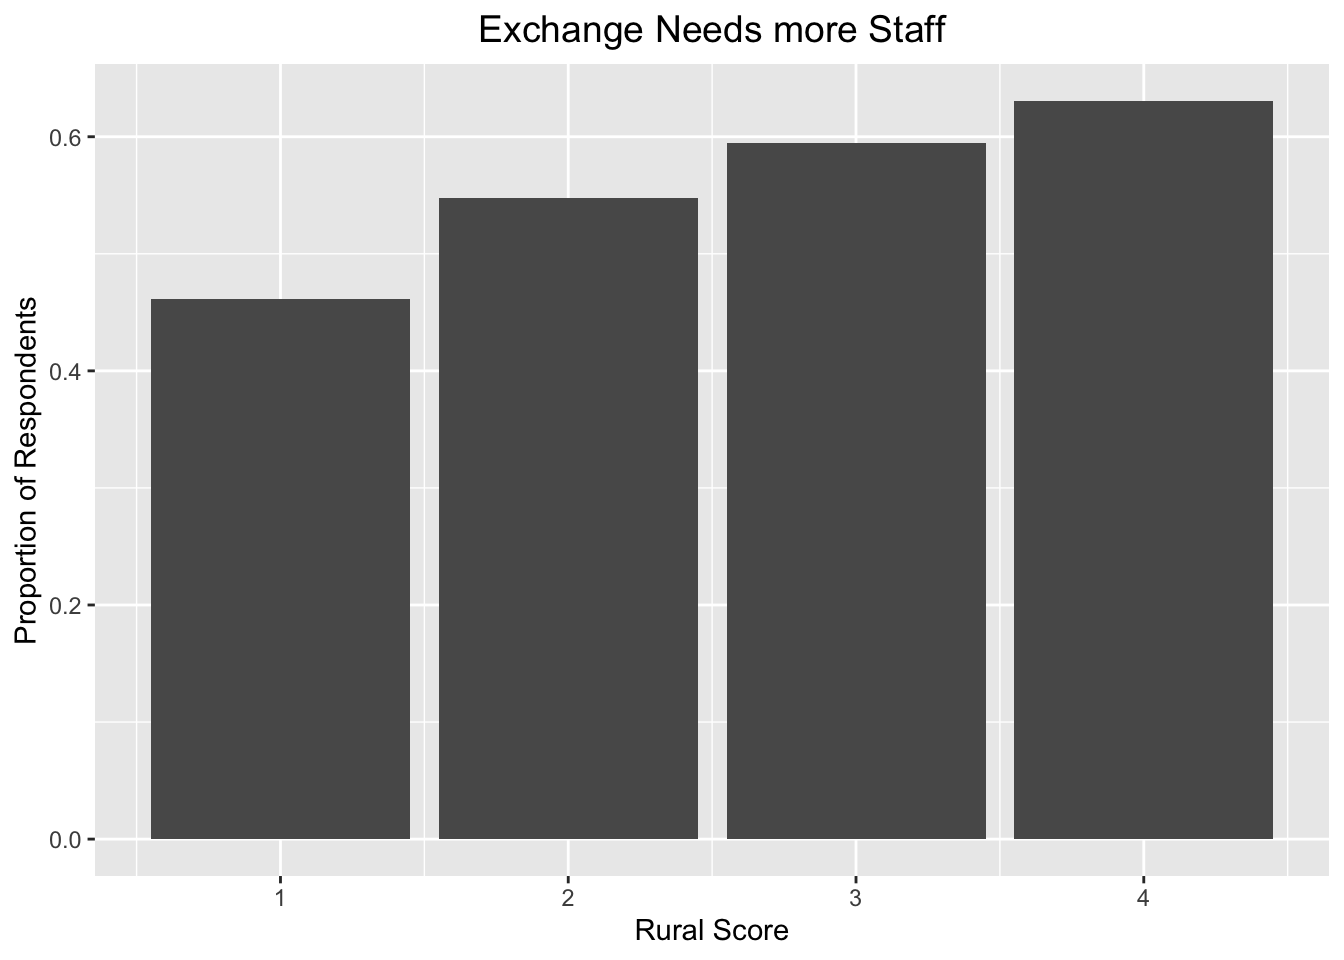
\includegraphics{coocli_files/figure-latex/unnamed-chunk-10-1.pdf}

\begin{verbatim}
## Cochran-Mantel-Haenszel Statistics for rural.fac by LawArrestedorConfiscatedSuppliesorCard 
## 
##                  AltHypothesis  Chisq Df       Prob
## cor        Nonzero correlation 11.044  1 0.00088975
## rmeans  Row mean scores differ 17.846  3 0.00047329
## cmeans  Col mean scores differ 11.044  1 0.00088975
## general    General association 17.846  3 0.00047329
\end{verbatim}

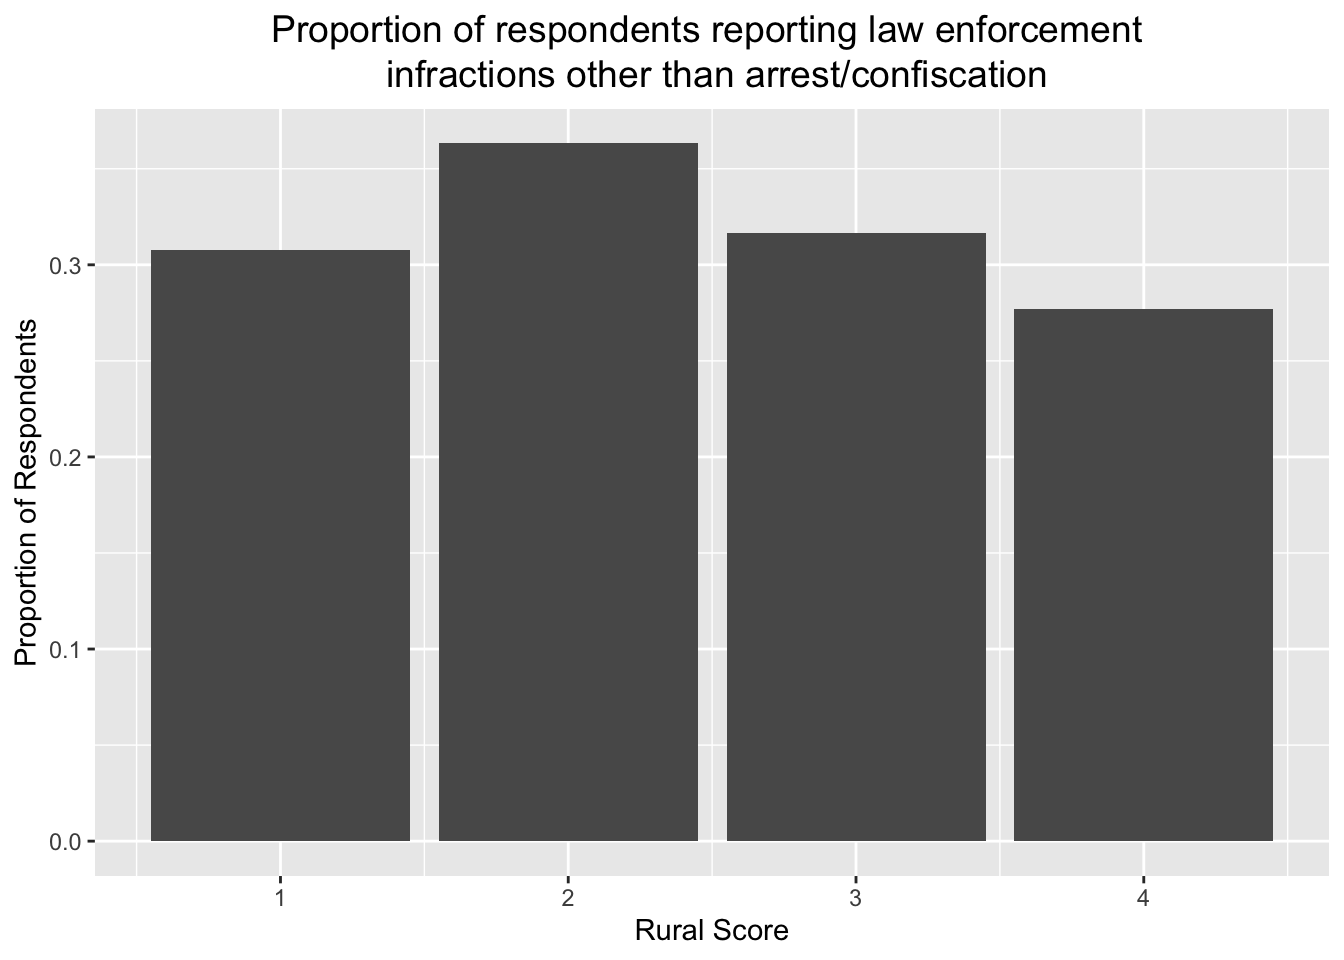
\includegraphics{coocli_files/figure-latex/unnamed-chunk-10-2.pdf}

\hypertarget{these-are-problems-specific-to-haywood-and-we-do-not-have-sufficient-data-to-claim-a-link-with-rurality-on-any-broader-scale.-one-thing-seems-clear---it-doesnt-seem-that-haywood-pd-are-behaving-this-way-out-of-ignorance---to-the-contrary-participants-in-haywood-did-not-report-that-officers-were-not-familiar-with-nchrc-at-any-notable-rate.-that-problem-officers-proclaimed-ignorance-of-nchrc-is-more-frequent-in-new-hanover-county-based-on-our-analysis.}{%
\subsubsection{\texorpdfstring{These are problems specific to Haywood, and we do not have sufficient data to claim a link with rurality on any broader scale. One thing seems clear - it doesn't seem that Haywood PD are behaving this way out of \emph{ignorance} - to the contrary, participants in Haywood \emph{did not} report that officers were \emph{not familiar} with NCHRC at any notable rate. That problem (officers' proclaimed ignorance of NCHRC) is more frequent in New Hanover county, based on our analysis.}{These are problems specific to Haywood, and we do not have sufficient data to claim a link with rurality on any broader scale. One thing seems clear - it doesn't seem that Haywood PD are behaving this way out of ignorance - to the contrary, participants in Haywood did not report that officers were not familiar with NCHRC at any notable rate. That problem (officers' proclaimed ignorance of NCHRC) is more frequent in New Hanover county, based on our analysis.}}\label{these-are-problems-specific-to-haywood-and-we-do-not-have-sufficient-data-to-claim-a-link-with-rurality-on-any-broader-scale.-one-thing-seems-clear---it-doesnt-seem-that-haywood-pd-are-behaving-this-way-out-of-ignorance---to-the-contrary-participants-in-haywood-did-not-report-that-officers-were-not-familiar-with-nchrc-at-any-notable-rate.-that-problem-officers-proclaimed-ignorance-of-nchrc-is-more-frequent-in-new-hanover-county-based-on-our-analysis.}}

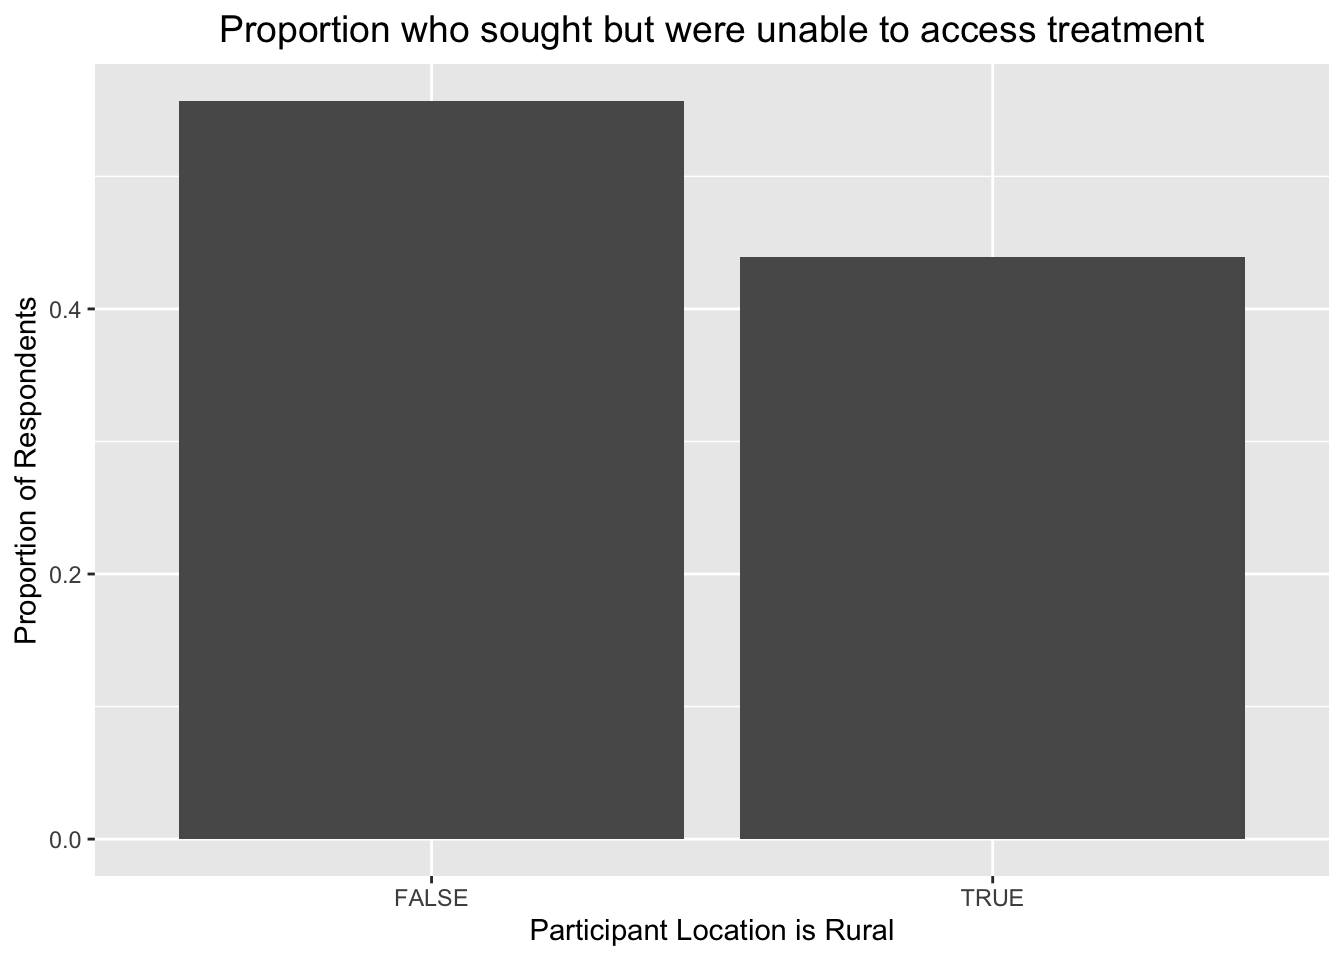
\includegraphics{coocli_files/figure-latex/unnamed-chunk-11-1.pdf}

\hypertarget{seems-inappropriate-to-attribute-any-difference-in-the-law-enforcement-questions-to-rurality-when-its-more-clearly-a-problem-with-haywood-and-most-specifically-a-problem-with-confiscation-ofarrest-for-supplies.}{%
\subsection{Seems inappropriate to attribute any difference in the law enforcement questions to rurality when it's more clearly a problem with Haywood, and most specifically a problem with confiscation of/arrest for supplies.}\label{seems-inappropriate-to-attribute-any-difference-in-the-law-enforcement-questions-to-rurality-when-its-more-clearly-a-problem-with-haywood-and-most-specifically-a-problem-with-confiscation-ofarrest-for-supplies.}}

With a more robust survey of participants, perhaps including more local measures of rurality (as opposed to a county-wide labeling approach), we might be able to learn more about how police departments differ in their education/training.

\hypertarget{one-peek-at-drug-use-profiles}{%
\chapter{One peek at drug-use profiles}\label{one-peek-at-drug-use-profiles}}

We lump substances into 5 groups, separating cocaine stimulants (powder, crack, speedball) from amphetamine stimulants (meth, adderall). We also separate MAT opioids from the other opioids. These groups create binary variables, giving no weight to those using multiple substances within a category. We have a fairly representative distribution of participants across the 5 groups, which are not mutually exclusive (someone can use MAT and stimulants for instance).

\hypertarget{those-on-medication-assisted-treatments-are-about-64-times-more-likely-to-express-interest-in-services-like-counseling-or-support-groups.}{%
\section{Those on Medication Assisted Treatments are about 64\% times more likely to express interest in services like counseling or support groups.}\label{those-on-medication-assisted-treatments-are-about-64-times-more-likely-to-express-interest-in-services-like-counseling-or-support-groups.}}

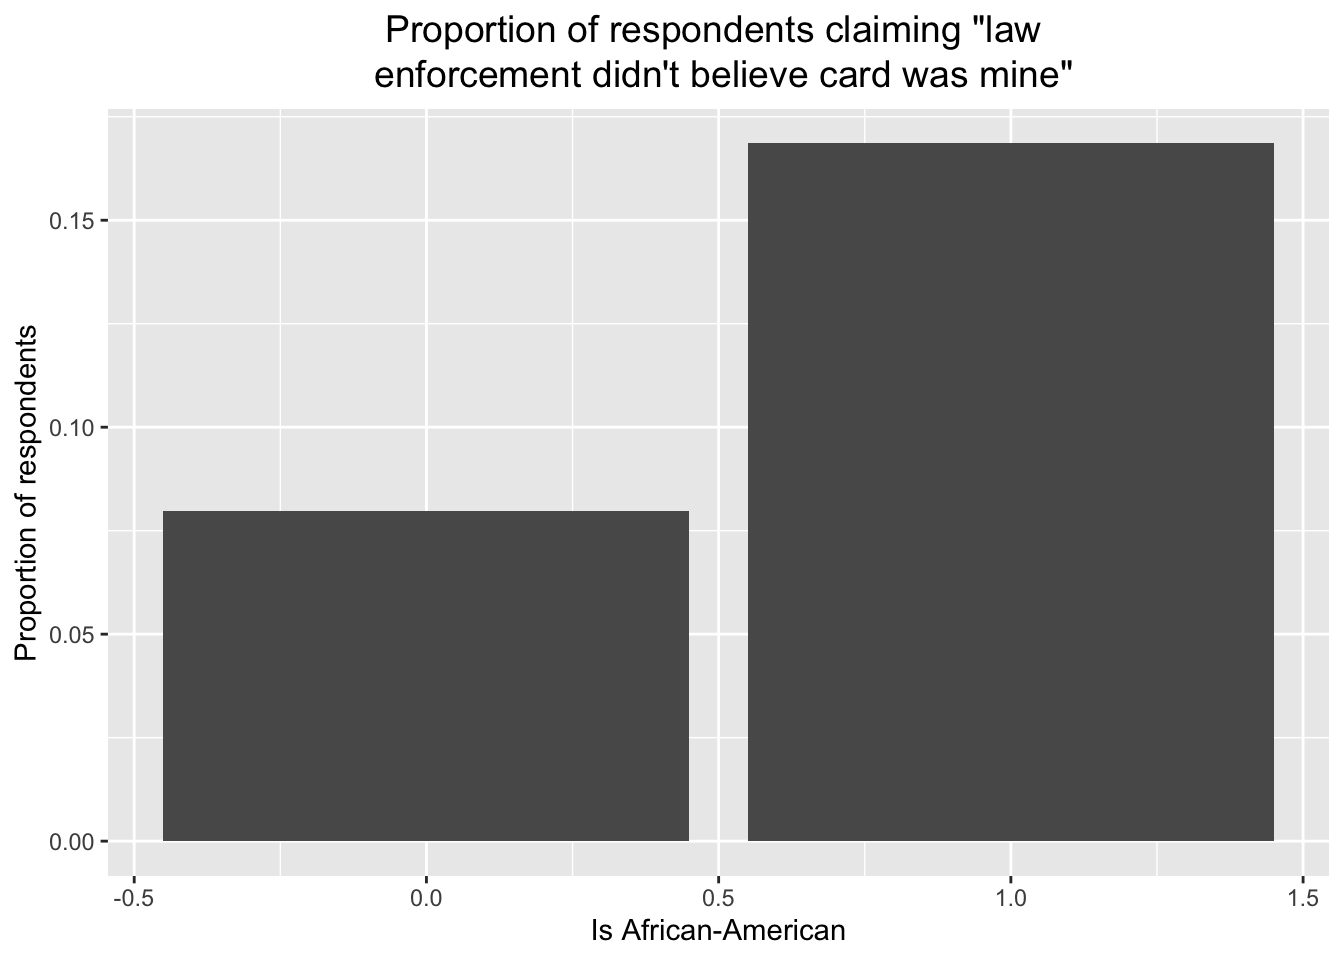
\includegraphics{coocli_files/figure-latex/unnamed-chunk-13-1.pdf}

\hypertarget{literature}{%
\chapter{Literature}\label{literature}}

Here is a review of existing methods.

\hypertarget{methods}{%
\chapter{Methods}\label{methods}}

We describe our methods in this chapter.

\hypertarget{applications}{%
\chapter{Applications}\label{applications}}

Some \emph{significant} applications are demonstrated in this chapter.

\hypertarget{example-one}{%
\section{Example one}\label{example-one}}

\hypertarget{example-two}{%
\section{Example two}\label{example-two}}

\hypertarget{final-words}{%
\chapter{Final Words}\label{final-words}}

We have finished a nice book.

\end{document}
